\section{Week 4 - Special applications: Face recognition \& Neural style transfer}
Discover how CNNs can be applied to multiple fields, including art generation and face recognition. Implement your own algorithm to generate art and recognize faces!

\subsection{Face Recognition}
Face verification vs. face recognition
\begin{itemize}
    \item \textbf{Verification}
    \begin{itemize}
        \item Input image, name/ID
        \item Output whether the input image is that of the claimed person
    \end{itemize}
\end{itemize}
\begin{itemize}
    \item \textbf{Recognition}
    \begin{itemize}
        \item Has a database of K persons
        \item Get an input image
        \item Output ID if the image is any of the K persons (or “not recognized”)
    \end{itemize}
\end{itemize}

\subsubsection{One Shot Learning}
One-shot learning problem; For most face recognition applications you need to be able to recognize a person given just one single image, or given just one example of that person's face.

The problen is you don't have enough dataset to get a CNN working, Learning from one example to recognize the person again.

Learning a “similarity” function wiht a NN
$d(img1,img2)$ = degree of difference between images for verification

\begin{equation*}
    \text{If } d(img1,img2) \left\{
                \begin{array}{ll}
                  \leq \pi \text{ same} \\
                  \ge \pi \text{ different}
                \end{array}
              \right. 
\end{equation*}

\subsubsection{Siamese Network}
Goal of learning
Parameters of NN define an encoding $f(x^{(i)})$ (a vector of sie 128). Learn the parameters so that:
\begin{itemize}
    \item if $x^{(i)}$, $x^{(j)}$ are the same person, $\left|\left|f(x^{(i)}) - f(x^{(j)})\right|\right|^2$ is small
    \item if $x^{(i)}$, $x^{(j)}$ are different persons, $\left|\left|f(x^{(i)}) - f(x^{(j)})\right|\right|^2$ is large
\end{itemize}

\subsubsection{Triplet Loss}
Learning Objective:
\begin{itemize}
    \item A: anchor
    \item P: positive
    \item N: negative
    \item $d(A, P) = \left|\left|f(A)-f(P)\right|\right|^2$
    \item $\alpha$ is a margin used to enusre the NN will not chose trivial solutions, e.g. $f(img)=0$ or any constant.
\end{itemize}
We want: 
\begin{equation}
    \left|\left|f(A)-f(P)\right|\right|^2 + \alpha \leq \left|\left|f(A)-f(N)\right|\right|^2
\end{equation}
\begin{equation}
    \left|\left|f(A)-f(P)\right|\right|^2 + \alpha - \left|\left|f(A)-f(N)\right|\right|^2 \leq 0
\end{equation}
Loss function:
Given 3 images A, P (same person as Anchor), N (different person than Anchor)
\begin{equation}
\mathcal{L}(A, P, N) = max (\left|\left|f(A)-f(P)\right|\right|^2 + \alpha - \left|\left|f(A)-f(N)\right|\right|^2, 0)
\end{equation}
So that the NN does not care how is the first part of max is negative.
\begin{equation}
J = \sum^m_{i=1} \mathcal{L}(A^{(i)}, P^{(i)}, N^{(i)})
\end{equation}

Training set: 10k pictures of 1k persons. If you have only one picture of this person then you cannot use this system.


Choosing the triplets A, P, N

During training, if A, P, N are chosen randomly, $d(A, P) + \alpha \leq d(A, N)$ is easily satisfied.

Choose triplets that're hard to train on, so that training algorith try hard to separate the two distances and avoid $d(A, P) \approx d(A, N)$

\subsubsection{Face Verification and Binary Classification}
Learning the similarity function

\begin{equation}
\hat{y} = \sigma(\sum^{128}_{k=1}w_i \left| f(x^{(i)})_k - f(x^{(j)})_k \right| + b)
\end{equation}
The input is a pair of images and the output is 0 or 1 dependening on whether you inputed similar pictures or not.

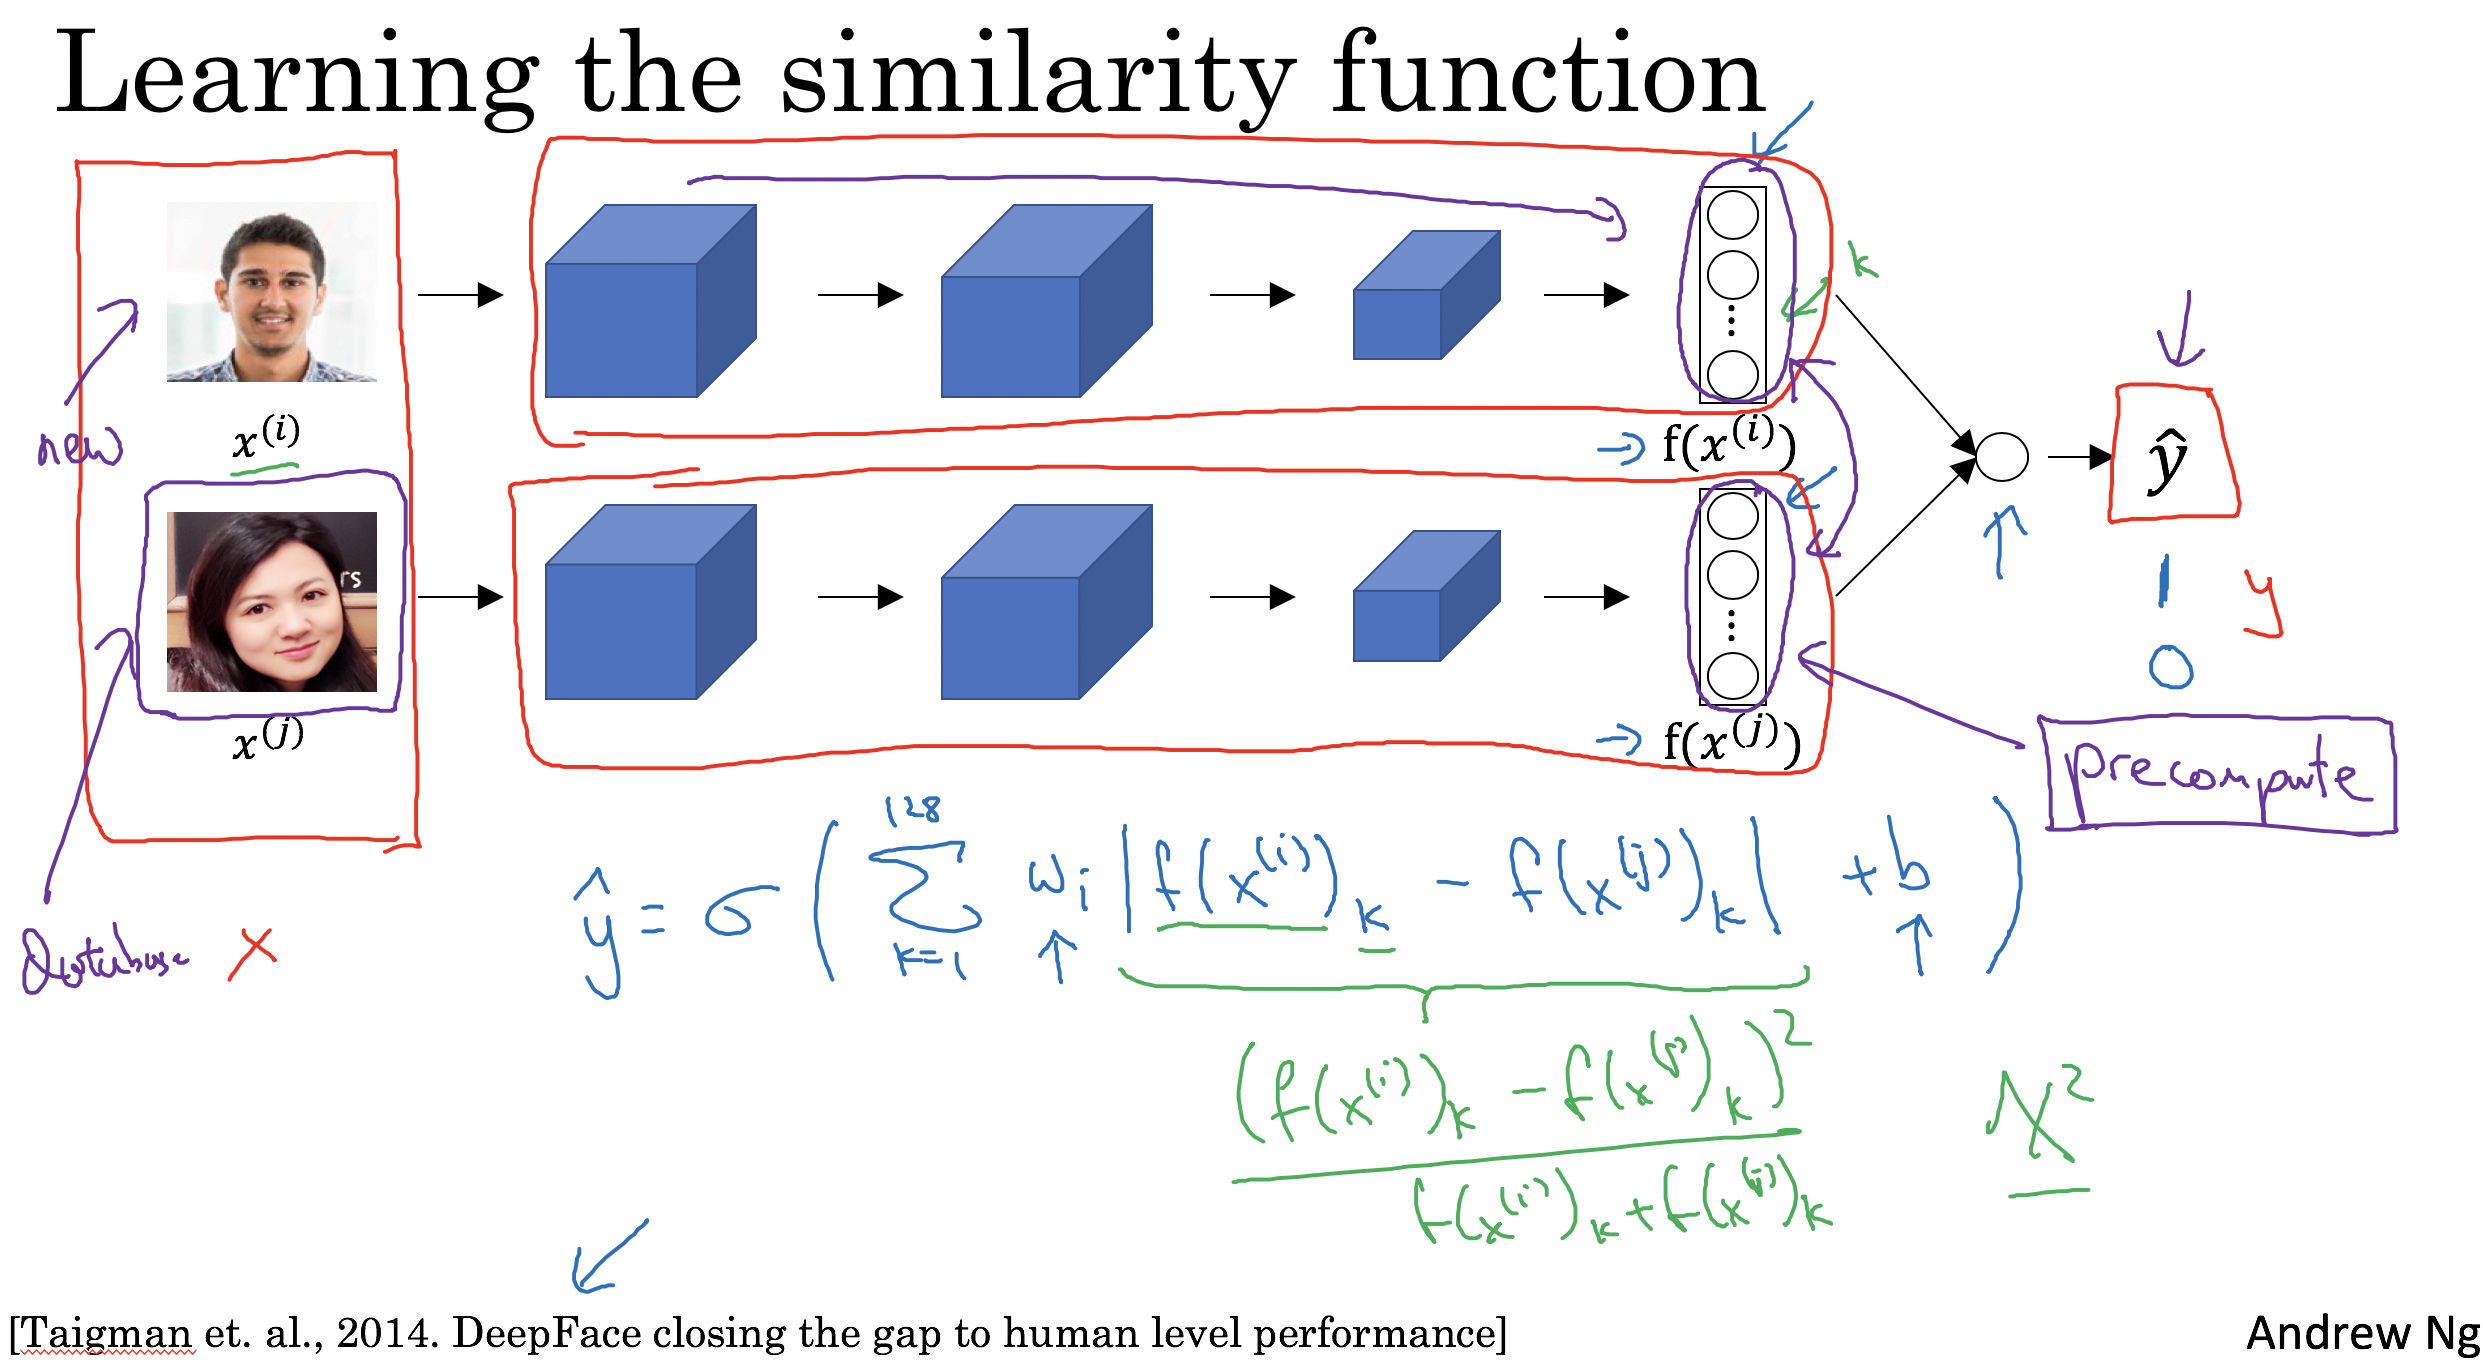
\includegraphics[scale=0.35]{Face_Verification}

\subsection{Neural Style Transfer}
\subsubsection{What is neural style transfer?}
Using an input picture C (Content) using a style image S (Style), combine them to generate a new image (G) in this style.

\subsubsection{What are deep ConvNets learning?}
Visualizing what a deep network is learning
Pick a unit in layer 1, Find the nine image patches that maximize the unit's activation.
Repeat for other units.

What you find for layer 1 is that it's learning shades, layer 2 it will looks for texture or complicated, etc.

\subsubsection{Cost Function}
To build a Neural style transfer algorithm we need to define a cost function that tells how good is the output image.
\begin{equation*}
    J(G) = \alpha J_{content}(C, G) + \beta J_{style} (S, G)
\end{equation*}
Algorithm to find the generated image G
\begin{enumerate}
    \item Initiate G randomly, G: 100 x 100 x 3
    \item Use gradient descent to minimize $J(G)$, $G = G - \frac{d}{dG} J(G)$
\end{enumerate}

\subsubsection{Content Cost Function}

\begin{equation}
    J(G) = \alpha J_{content} (C, G) + \beta J_{style} (S, G)
\end{equation}

\begin{itemize}
    \item Say you use hidden layer $l$ to compute content cost. 
    \item Use pre-trained ConvNet. (E.g., VGG network)
    \item Let $a^{[l](C)}$ and $a^{[l](G)}$ be the activation of layer $l$ on the images   
    \item if $a^{[l](C)}$  and $a^{[l](G)}$ are similar, both images have similar content.
\end{itemize}
\begin{equation}
J_{content}(C, G) = \frac{1}{2} \left|\left| a^{[l](C)} - a^{[l](G)} \right|\right|^2
\end{equation}

\begin{quote}
     But it's really just the element-wise sum of squares of differences between the activations in layer l, between the images in C and G. And so, when later you perform gradient descent on J(G) to try to find a value of G, so that the overall cost is low, this will incentivize the algorithm to find an image G, so that these hidden layer activations are similar to what you got for the content image.
\end{quote}

\subsubsection{Style Cost Function}
Meaning of the style of an image

Say you are using layer $l$'s activation to measure "style". Define "style" as \textbf{correlation} between activations across channels.

How correlated are the activations across different channels? How often they occur together in parts of an image or not. If we use the degree of correction across channels of an image, then we can do is compute the degree of correction in the generated image this channel is correlated. This will tells you how often in the generated image a given texture occurs.

Style matrix

Let $a^{[l]}_{i,j,k}$ = activation at (i, j, k), i.e. height, width, channel. $G^{[l]}$ is $n^{[l]}_{c}$ x $n^{[l]}_{c}$

For the style image, compute the non normalized loss function as follows:
\begin{equation*}
G^{[l](S)}_{kk'} = \sum^{n^{[l]}_h}_{i=1} \sum^{n^{[l]}_{w}}_{j=1} a^{[l](S)}_{i,j,k} a^{[l](S)}_{i,j,k'}
\end{equation*}
For the generated image, compute the non normalized loss function as follows:
\begin{equation*}
G^{[l](G)}_{kk'} = \sum^{n^{[l]}_h}_{i=1} \sum^{n^{[l]}_{w}}_{j=1} a^{[l](G)}_{i,j,k} a^{[l](G)}_{i,j,k'}
\end{equation*}

\begin{equation*}
J^{[l]}_{style} (S, G) = \left|\left| G^{[l](S)} - G^{[l](G)} \right|\right|^2_F
\end{equation*}

Style cost function at layer $l$

\begin{equation*}
J^{[l]}_{style} (S, G) = \frac{1}{(2n^{[l]}_H n^{[l]}_W n^{[l]}_C)^2} \sum_{k} \sum_{k'} (G^{[l](S)}_{kk'} - G^{[l](G)}_{kk'})
\end{equation*}

Summing up at all layers, the overal cost function becomes;
\begin{equation*}
J_{style} (S, G) = \sum_l \lambda^{[l]} J^{[l]}_{style} (S, G)
\end{equation*}

\subsubsection{1D and 3D Generalizations}
You have learned a lot about ConvNets, everything ranging from the architecture of the ConvNet to how to use it for image recognition, to object detection, to face recognition and neural-style transfer. 

Many of the ideas we learned here can be applied to 1D or 3D data, not just images.


\subsection{Practice questions}
\subsubsection{QUIZ - Special applications: Face recognition \& Neural style transfer}
\textbf{1.} Face verification requires comparing a new picture against one person’s face, whereas face recognition requires comparing a new picture against K person’s faces.
\begin{itemize}
    \item True (X)
    \item False
\end{itemize}
\textbf{2.} Why do we learn a function $d(img1, img2)$ for face verification? (Select all that apply.)
\begin{itemize}
    \item Given how few images we have per person, we need to apply transfer learning.
    \item This allows us to learn to recognize a new person given just a single image of that person. (X)
    \item We need to solve a one-shot learning problem. (X)
    \item This allows us to learn to predict a person’s identity using a softmax output unit, where the number of classes equals the number of persons in the database plus 1 (for the final “not in database” class).
\end{itemize}
\textbf{3.} In order to train the parameters of a face recognition system, it would be reasonable to use a training set comprising 100,000 pictures of 100,000 different persons.
\begin{itemize}
    \item True
    \item False (X)
\end{itemize}
\textbf{4.} Which of the following is a correct definition of the triplet loss? Consider that $\alpha > 0$. (We encourage you to figure out the answer from first principles, rather than just refer to the lecture.)
\begin{itemize}
    \item $max(\left|\left| f(A) - f(P) \right|\right|^2 - \left|\left| f(A) - f(N) \right|\right|^2 - \alpha, 0)$
    \item $max(\left|\left| f(A) - f(N) \right|\right|^2 - \left|\left| f(A) - f(P) \right|\right|^2 - \alpha, 0)$
    \item $max(\left|\left| f(A) - f(N) \right|\right|^2 - \left|\left| f(A) - f(P) \right|\right|^2 + \alpha, 0)$
    \item $max(\left|\left| f(A) - f(P) \right|\right|^2 - \left|\left| f(A) - f(N) \right|\right|^2 + \alpha,0)$ (X)
\end{itemize}
\textbf{5.} Consider the following Siamese network architecture:

The upper and lower neural networks have different input images, but have exactly the same parameters.
\begin{itemize}
    \item True
    \item False
\end{itemize}
\textbf{6.} You train a ConvNet on a dataset with 100 different classes. You wonder if you can find a hidden unit which responds strongly to pictures of cats. (I.e., a neuron so that, of all the input/training images that strongly activate that neuron, the majority are cat pictures.) You are more likely to find this unit in layer 4 of the network than in layer 1.
\begin{itemize}
    \item True (X)
    \item False
\end{itemize}
\textbf{7.} Neural style transfer is trained as a supervised learning task in which the goal is to input two images ($x$), and train a network to output a new, synthesized image ($y$).
\begin{itemize}
    \item True
    \item False (X)
\end{itemize}
\textbf{8.} In the deeper layers of a ConvNet, each channel corresponds to a different feature detector. The style matrix $G^{[l]}$  measures the degree to which the activations of different feature detectors in layer $l$ vary (or correlate) together with each other.
\begin{itemize}
    \item True (X)
    \item False
\end{itemize}
\textbf{9.} In neural style transfer, what is updated in each iteration of the optimization algorithm?
\begin{itemize}
    \item The neural network parameters
    \item The pixel values of the generated image $\mathcal{G}$ (X)
    \item The pixel values of the content image $\mathcal{C}$
    \item The regularization parameters
\end{itemize}
\textbf{10.} You are working with 3D data. You are building a network layer whose input volume has size 32x32x32x16 (this volume has 16 channels), and applies convolutions with 32 filters of dimension 3x3x3 (no padding, stride 1). What is the resulting output volume?
\begin{itemize}
    \item 30x30x30x32 (X)
    \item 30x30x30x16
    \item Undefined: This convolution step is impossible and cannot be performed because the dimensions specified don’t match up.
\end{itemize}